\documentclass{article}
\usepackage{graphicx} % Required for inserting images
\usepackage{amssymb}
\usepackage{amsmath}
\usepackage{amsfonts}
%\usepackage{extarrows}
\usepackage{soul}
\tolerance=1
\emergencystretch=\maxdimen
\hyphenpenalty=10000
\hbadness=10000
\let\oldemptyset\emptyset
\usepackage[T1]{fontenc}

\author{Amnézic}
\date{}
\title{Modèle OSI}

\begin{document}
\maketitle
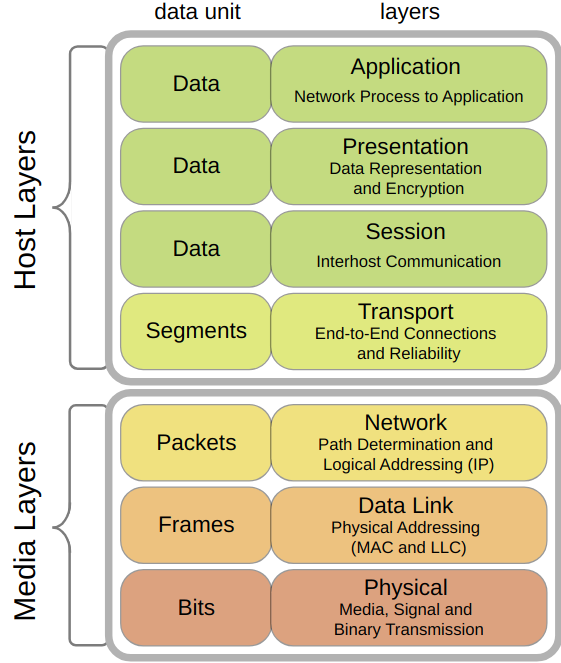
\includegraphics[scale=0.5]{OSI_model.png}
\newpage
\tableofcontents
\newpage

\section{Introduction}
Le modèle d'Interconnexion des systèmes ouverts (\textit{Open Systems Interconnection model} en anglais) est un modèle conceptuel de l'ISO qui permet d'obtenir une base commune pour la coordination des standards dans le développement des systèmes internconnectés. Ce modèle est constitué de sept niveaux que nous développerons par la suite. En clair, ce modèle permet de découpé un système de comunication en plusieurs parties afin de mieux les comprendre et les mettre en place. Ce modèle est un incoutournable dans le domaine du développement de logiciels car il est la base de chaque projet software. Il permet mettre en place des règles pour la communications entre ordinateurs, du bit jusqu'aux paquets de données.


\section{Sujets annexes à regarder :}

\end{document}